\documentclass[tikz,border=8pt]{standalone}
\usetikzlibrary{arrows.meta,positioning,decorations.pathmorphing}
\begin{document}
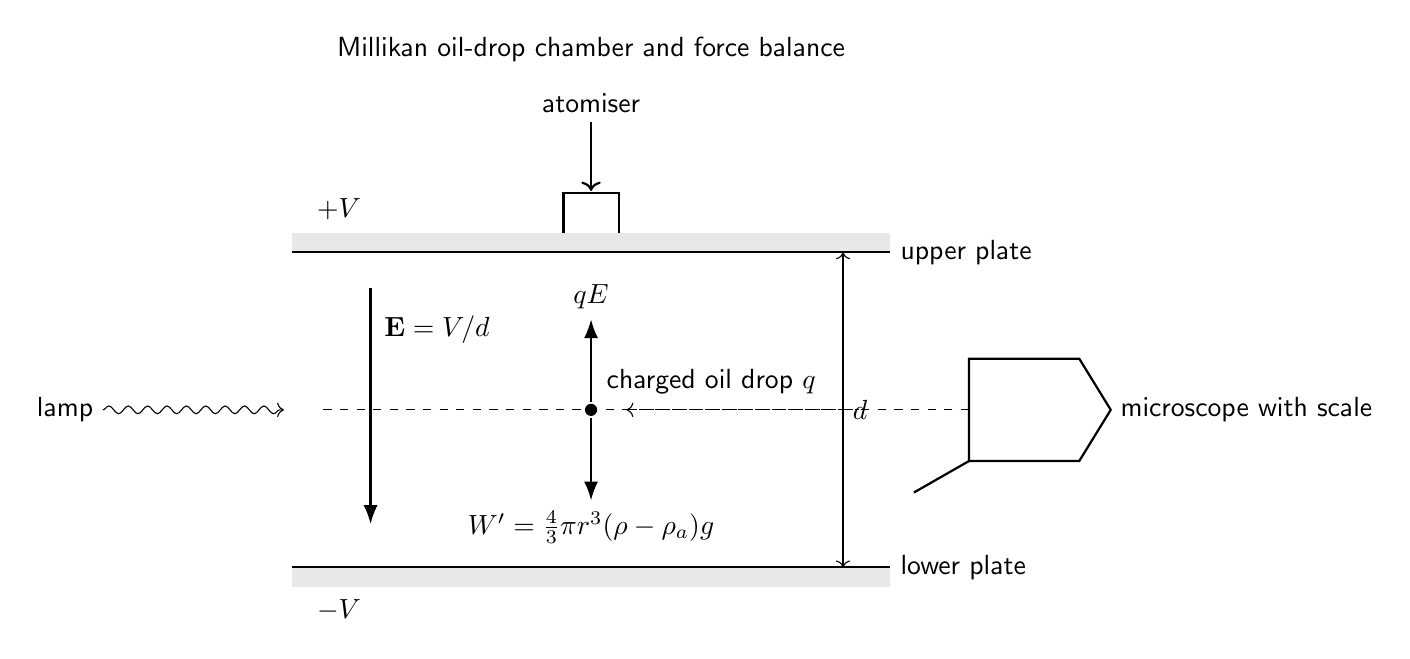
\begin{tikzpicture}[font=\sffamily, force/.style={-{Latex[length=2.4mm]},thick}]
  \fill[gray!18] (-3.8,2.0) rectangle (3.8,2.25);
  \fill[gray!18] (-3.8,-2.0) rectangle (3.8,-2.25);
  \draw[thick] (-3.8,2.0) -- (3.8,2.0) node[right]{upper plate};
  \draw[thick] (-3.8,-2.0) -- (3.8,-2.0) node[right]{lower plate};
  \draw[dashed] (-3.4,0) -- (3.4,0);
  \node at (-3.2,2.55) {$+V$};
  \node at (-3.2,-2.55) {$-V$};
  \draw[force] (-2.8,1.55) -- (-2.8,-1.45);
  \node[above right] at (-2.75,.72) {$\mathbf E=V/d$};

  \fill (0,0) circle (2.2pt) node[above right=3pt]{charged oil drop $q$};
  \draw[force] (0,.1) -- (0,1.15) node[above]{$qE$};
  \draw[force] (0,-.1) -- (0,-1.15) node[below]{$W'=\frac43\pi r^3(\rho-\rho_a)g$};

  \draw[thick] (-.35,2.25) -- (-.35,2.75) -- (.35,2.75) -- (.35,2.25);
  \draw[->,thick] (0,3.65) -- (0,2.78);
  \node[above] at (0,3.65) {atomiser};

  \draw[thick] (4.8,.65) -- (6.2,.65) -- (6.6,0) -- (6.2,-.65) -- (4.8,-.65) -- cycle;
  \draw[thick] (4.8,-.65) -- (4.1,-1.05);
  \node[right] at (6.6,0) {microscope with scale};
  \draw[dashed,->] (4.8,0) -- (.45,0);

  \draw[decorate,decoration={snake,amplitude=1.4pt,segment length=7pt},->] (-6.2,0) -- (-3.9,0);
  \node[left] at (-6.2,0) {lamp};
  \draw[<->] (3.2,-2.0) -- (3.2,2.0) node[midway,right]{$d$};
  \node[above] at (0,4.3) {Millikan oil-drop chamber and force balance};
\end{tikzpicture}
\end{document}
